\section*{Dati e risultati}

\subsection*{Circuito invertente}

Il primo circuito studiato sfrutta l'opamp LM741 al fine di amplificare e sfasare di $180^\circ$ il segnale in ingresso ($V\ped{in}$). Il circuito che abbiamo realizzato è illustrato in Figura \ref{fig:amp_inv}.
Questo circuito è alimentato con una tensione costante positiva di $\SI{+15}{\volt}$ e una negativa di $\SI{-15}{\volt}$, un segnale in ingresso variabile ($V\ped{in}$) ottenuto grazie al generatore di onde.
Dal momento che vogliamo che tale circuito abbia un guadagno ($G$) di circa 10 dobbiamo dimensionarlo. In particolare sappiamo che in questo caso vale la relazione:

\begin{equation}
        G\,=\,-\frac{V\ped{out}}{V\ped{in}}\,=\,-\frac{R_2}{R_1} \qquad => \qquad |R_2|\,=\,10\,|R_1|
        \label{eq:g}
\end{equation}

dove $R_1$ e $R_2$ sono le resistenze del circuito in analisi, $V\ped{in}$ il segnale in ingresso e $V\ped{out}$ il segnale in uscita. Quindi, per non avere intensità di correnti troppo elevate all'interno del circuito, abbiamo deciso di porre $R_2\,=\,\SI{100}{\kilo\ohm}$ e $R_1\,=\,\SI{10}{\kilo\ohm}$.

Fatto questo abbiamo verificato che il guadagno di tale circuito, a frequenza fissta $\nu\,=\,\SI{1}{\kilo\hertz}$, fosse costante. A tal fine abbiamo misurato $V\ped{out}$ al variare dell'ampiezza del segnale in ingresso $V\ped{in}$. Pertanto sfruttando la relazione (\ref{eq:g}) abbiamo fatto la media dei valori di $G$ così ricavati e abbiamo ottenuto che il guadagno del nostro circuito vale:

\begin{equation}
        G\,=\, XXX
\end{equation}

Successivamente abbiamo deciso di studiare come varia il guadagno al variare della frequenza di $V\ped{in}$, mantenendo costante l'ampiezza di $V\ped{in}$. Quello che abbiamo ottenuto è riportato in Figura \ref{fig:g_vs_freq}

\begin{figure}
    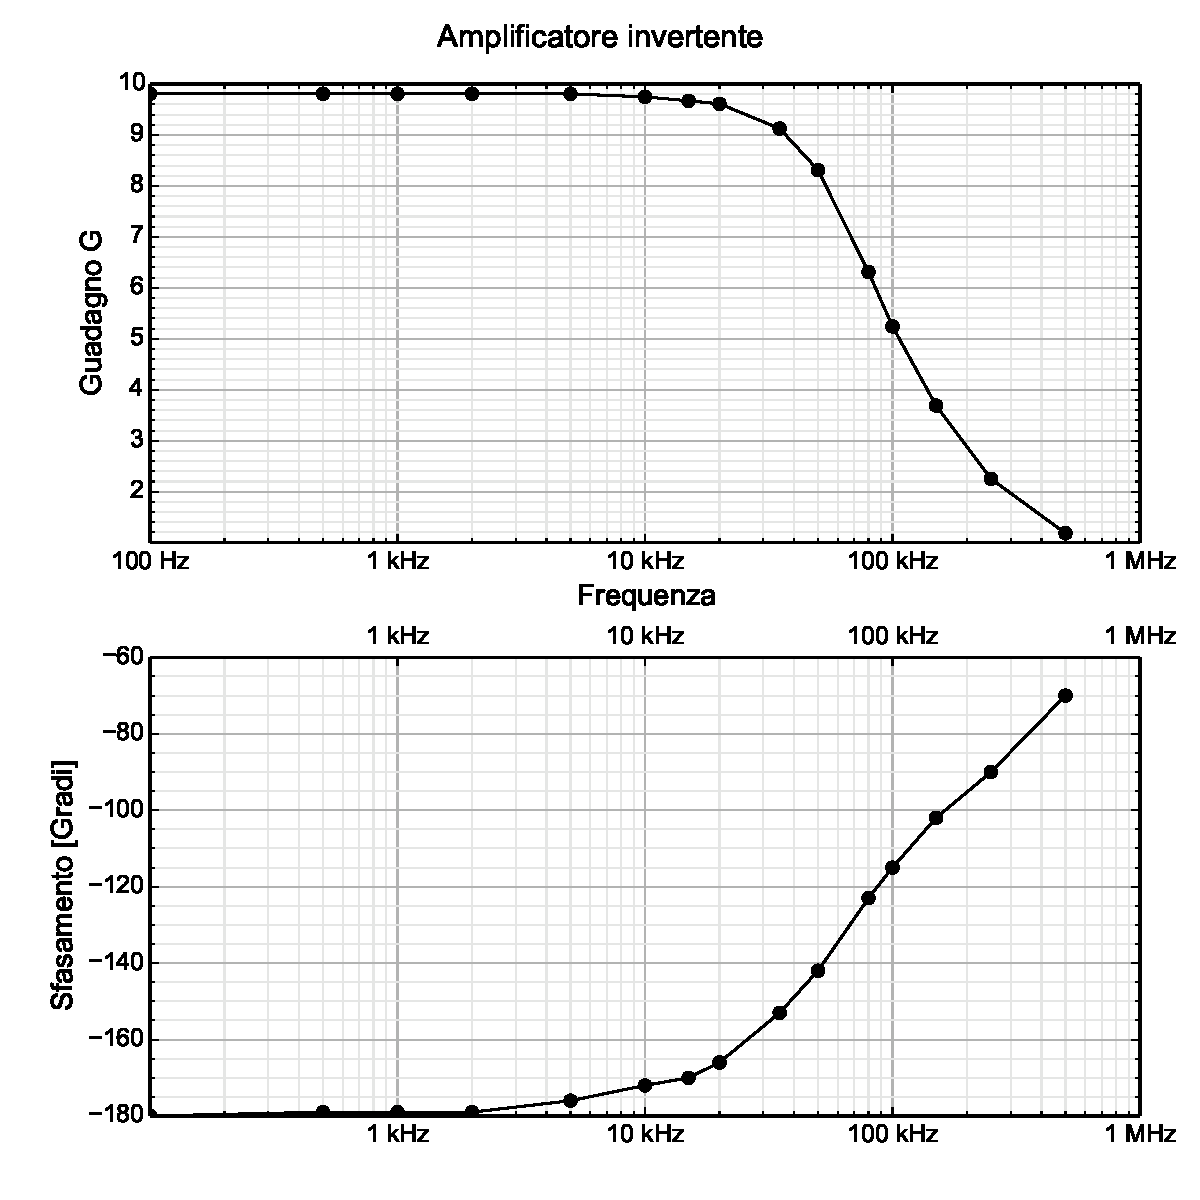
\includegraphics[width=0.75\textwidth]{amp_inv.pdf}
    \label{fig:g_vs_freq}
\end{figure}

Infine abbiamo trovato i valori di ampiezza del segnale in uscita $V\ped{out}$, a frequenza costante $\nu\,=\,\SI{1}{\kilo\hertz}$ di $V\ped{in}$, per i quali si verifica il fenomeno del clamping. Tali valori sono risultati essere:

\begin{equation}
        V\ped{out}^+\,\simeq\,\SI{14.2}{\volt} \qquad \text{e} \qquad V\ped{out}^-\,\simeq\,\SI{-13.1}{\volt}
\end{equation}

\subsection*{Circuito non invertente}

Questo circuito, come il precedente, sfrutta l'op-amp 471 al fine di ottenere un'amplificazione del segnale in ingresso $V\ped{in}$, ma in questo caso non è presente uno sfasamento di $180^\circ$ tra i due segnali ($V\ped{in}$ e $V\ped{out}$).
Il circuito utilizzato è riportato in Figura \ref{fig:amp_noninv}. Le sue specifiche sono esattamente uguali a quelle del circuito descritto in precedenza a parte il fatto che le due resistenze $R_1$ e $R_2$ sono posizionate in punti differenti del circuito.
Anche in questo caso abbiamo svolto delle misure di $V\ped{out}$ in funzione di $V\ped{in}$, mantenedo costante la frequenza $\nu\,=\,\SI{1}{\kilo\hertz}$ di $V\ped{in}$, e abbiamo ottenuto, grazie all'equazione (\ref{eq:g}), che:

\begin{equation}
        G\,=\, XXX
\end{equation}

Successivamente abbiamo valutato l'andamento di $V\ped{out}$ in funzione della frequenza ($\nu$) di $V\ped{in}$ e abbiamo ottenuto quanto illustrato in Figura \ref{fig:} sempre sfruttando la relazione vista in (\ref{eq:g})

Infine, come nell'analisi dl circuito precedente, abbiamo trovato i valori di ampiezza del segnale in uscita $V\ped{out}$, a frequenza costante $\nu\,=\,\SI{1}{\kilo\hertz}$ di $V\ped{in}$, per i quali si verifica il fenomeno del clamping. Tali valori sono risultati essere:

\begin{equation}
        V\ped{out}^+\,\simeq\,\SI{}{\volt} \qquad \text{e} \qquad V\ped{out}^-\,\simeq\,\SI{}{\volt}
\end{equation}

\subsection*{Circuito sommatore}
















